\documentclass[journal,12pt,twocolumn]{IEEEtran}

\usepackage{setspace}
\usepackage{gensymb}
\singlespacing
\usepackage[cmex10]{amsmath}
\usepackage{cancel}
\usepackage{amsthm}
\usepackage{amsmath}
\usepackage{paralist}
\usepackage{upgreek}
\usepackage{mathrsfs}
\usepackage{txfonts}
\usepackage{stfloats}
\usepackage{bm}
\usepackage{cite}
\usepackage{cases}
\usepackage{subfig}

\usepackage{longtable}
\usepackage{multirow}
\usepackage{enumitem}
\usepackage{mathtools}
\usepackage{steinmetz}
\usepackage{tikz}
\usepackage{circuitikz}
\usepackage{verbatim}
\usepackage{tfrupee}
\usepackage[breaklinks=true]{hyperref}
\usepackage{graphicx}
\usepackage{tkz-euclide}

\usetikzlibrary{calc,math}
\usepackage{listings}
    \usepackage{color}                                            %%
    \usepackage{array}                                            %%
    \usepackage{longtable}                                        %%
    \usepackage{calc}                                             %%
    \usepackage{multirow}                                         %%
    \usepackage{hhline}                                           %%
    \usepackage{ifthen}                                           %%
    \usepackage{lscape}     
\usepackage{multicol}
\usepackage{chngcntr}

\DeclareMathOperator*{\Res}{Res}
\usepackage{romannum}
\renewcommand\thesection{\arabic{section}}
\renewcommand\thesubsection{\thesection.\arabic{subsection}}
\renewcommand\thesubsubsection{\thesubsection.\arabic{subsubsection}}

\renewcommand\thesectiondis{\arabic{section}}
\renewcommand\thesubsectiondis{\thesectiondis.\arabic{subsection}}
\renewcommand\thesubsubsectiondis{\thesubsectiondis.\arabic{sub subsection}}
\newtheorem{theorem}{Theorem}[section]
\newtheorem{corollary}{Corollary}[theorem]
\newtheorem{lemma}[theorem]{Lemma}
\newtheorem{definition}{Definition}[section]


\hyphenation{optical networks semiconduc-tor}
\def\inputGnumericTable{}                                 %%

\lstset{
%language=C,
frame=single, 
breaklines=true,
columns=fullflexible
}
\date{March 2021}

\begin{document}
\newcommand{\multlinecomment}[1]{\directlua{-- #1}}
\newcommand{\BEQA}{\begin{eqnarray}}
\newcommand{\EEQA}{\end{eqnarray}}
\newcommand{\define}{\stackrel{\triangle}{=}}
\bibliographystyle{IEEEtran}
\raggedbottom
\setlength{\parindent}{0pt}
\providecommand{\mbf}{\mathbf}
\providecommand{\pr}[1]{\ensuremath{\Pr\left(#1\right)}}
\providecommand{\qfunc}[1]{\ensuremath{Q\left(#1\right)}}
\providecommand{\fn}[1]{\ensuremath{f\left(#1\right)}}
\providecommand{\e}[1]{\ensuremath{E\left(#1\right)}}
\providecommand{\sbrak}[1]{\ensuremath{{}\left[#1\right]}}
\providecommand{\lsbrak}[1]{\ensuremath{{}\left[#1\right.}}
\providecommand{\rsbrak}[1]{\ensuremath{{}\left.#1\right]}}
\providecommand{\brak}[1]{\ensuremath{\left(#1\right)}}
\providecommand{\lbrak}[1]{\ensuremath{\left(#1\right.}}
\providecommand{\rbrak}[1]{\ensuremath{\left.#1\right)}}
\providecommand{\cbrak}[1]{\ensuremath{\left\{#1\right\}}}
\providecommand{\lcbrak}[1]{\ensuremath{\left\{#1\right.}}
\providecommand{\rcbrak}[1]{\ensuremath{\left.#1\right\}}}
\theoremstyle{remark}
\newtheorem{rem}{Remark}
\newcommand{\sgn}{\mathop{\mathrm{sgn}}}
\providecommand{\abs}[1]{\vert#1\vert}
\providecommand{\res}[1]{\Res\displaylimits_{#1}} 
\providecommand{\norm}[1]{\lVert#1\rVert}
%\providecommand{\norm}[1]{\lVert#1\rVert}
\providecommand{\mtx}[1]{\mathbf{#1}}
\providecommand{\mean}[1]{E[ #1 ]}
\providecommand{\fourier}{\overset{\mathcal{F}}{ \rightleftharpoons}}
%\providecommand{\hilbert}{\overset{\mathcal{H}}{ \rightleftharpoons}}
\providecommand{\system}{\overset{\mathcal{H}}{ \longleftrightarrow}}
	%\newcommand{\solution}[2]{\textbf{Solution:}{#1}}
\newcommand{\solution}{\noindent \textbf{Solution: }}
\newcommand{\cosec}{\,\text{cosec}\,}
\providecommand{\dec}[2]{\ensuremath{\overset{#1}{\underset{#2}{\gtrless}}}}
\newcommand{\myvec}[1]{\ensuremath{\begin{pmatrix}#1\end{pmatrix}}}
\newcommand{\mydet}[1]{\ensuremath{\begin{vmatrix}#1\end{vmatrix}}}
\numberwithin{equation}{subsection}
\makeatletter
\vspace{3cm}
\title{Quiz-2}
\author{Savarana Datta Reddy - AI20BTECH11008}
\maketitle
\newpage
\bigskip
\renewcommand{\thetable}{\theenumi}

%
Download latex code from 
%
\begin{lstlisting}
https://github.com/SavaranaDatta/EE900/tree/main/Quiz2
\end{lstlisting}

\section{Question}
For the following pair of input $z$-transform $X(z)$ and system function $H(z)$, determine the region of convergence for the output $z$-transform $Y(z)$:
\begin{align}
    X(z)&=\frac{1}{\brak{1-\frac{1}{5}{z^{-1}}}\brak{1+3z^{-1}}},\hspace{0.4cm}  \frac{1}{5}<|z|<3\\
    H(z)&=\frac{1+3z^{-1}}{1+\frac{1}{3}z^{-1}}, \hspace{2cm} |z|>\frac{1}{3}
\end{align}
\section{Solution}
\begin{lemma}{\textbf{Properties of ROC:}}
The ROC doesnot contain any poles.\\
For
\begin{align}
    X(s)=\frac{N(s)}{D(s)}
\end{align}
The poles of X(s)\implies D(s)=0
\end{lemma}
\begin{lemma}
 The poles of X(s) consists of a strip parallel to j$\omega$ axis in the s-plane.
\end{lemma}
We know that the $z$-transform of output signal ($Y(z)$)
\begin{align}
    Y(z)=H(z)X(z)
\end{align}
Here
\begin{align}
    Y(z)&=\brak{\frac{1}{\brak{1-\frac{1}{5}{z^{-1}}}\brak{1+3z^{-1}}}} \brak{\frac{1+3z^{-1}}{1+\frac{1}{3}z^{-1}}}\\
        &= \frac{1}{\brak{1-\frac{1}{5}{z^{-1}}}\brak{1+\frac{1}{3}z^{-1}}} \label{eq1}\\
        &= 1 - \frac{5}{24\brak{z+\frac{1}{3}}}+\frac{3}{40\brak{z-\frac{1}{5}}}, \hspace{1cm} \frac{1}{3}<|z|<3
\end{align}
The poles of $Y(z)$ are 
\begin{align}
    z=\frac{-1}{3}, \frac{1}{5}
\end{align}
The zeros of $Y(z)$ are 
\begin{align}
    z=0
\end{align}

 From the above 2 lemmas we can say that the possible ROCs of
 \begin{align}
     Y(z)= \frac{1}{\brak{1-\frac{1}{5}{z^{-1}}}\brak{1+\frac{1}{3}z^{-1}}} 
 \end{align}
 are 
 \begin{align}
     z<\frac{-1}{3}\\
     \frac{-1}{3}<z<\frac{1}{5}\\
     z>\frac{1}{5}
 \end{align}
 But this expression of $Y(z)$ is valid for the interval $\frac{1}{3}<|z|<3$. Hence, the ROC of $Y(z)$ is $z>\frac{1}{3}$ and $z<\frac{-1}{3}$ i.e, $|z|>\frac{1}{3}$.
\begin{figure}[htp]
    \centering
    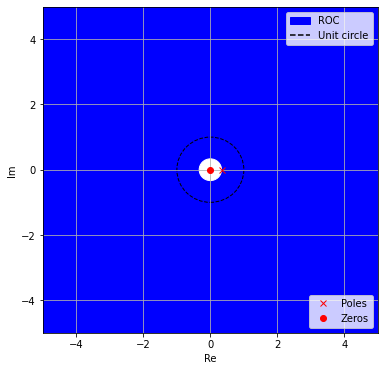
\includegraphics[width=\columnwidth]{fig1.png}
    \caption{ploe-zero plot of the system}
\end{figure}
\end{document}
